\section{Expert-based knowledge}
    \subsection{Expert-based approach}
        The expert-based approach is based on the domain knowledge of the fraud analyst: he is able to gather and process the right information in the right manner.\\
        Performing detailed and manual investigation of suspicious cases, may indicate a new fraud mechanism, an analyst can understand and address the new mechanism.\\
        Comprehension of the fraud mechanism allows extending the fraud detection and prevention mechanism.\\ 
        Every time a new transaction is flagged suspicious, is going to be investigated, if it's labeled as fraud, the specific case will be added to the fraud detection mechanism.
    \subsection{Fraud investigation and management}
        There are two possible types of measures that can be taken when fraudulent activities are detected and confirmed:
        \begin{itemize}
            \item Corrective Measures
            \item Preventive Measures
        \end{itemize}
        \subsubsection{Corrective Measures} 
            Aim to resolve the fraud and correct the consequences. We call \textbf{retrospective screening} the set of actions to retrospectively detect frauds and subsequently address similar cases.\\
            The sooner corrective measures are taken and fraud is detected, the more effective such measures are and the more losses can be avoided.
        \subsubsection{Preventive Measures}
            Aim to prevent future frauds, making the organization more robust and less vulnerable.\\
            The typical process:
            \begin{itemize}
                \item Investigate the fraud case to understand the underlying mechanisms
                \item Extend the available expert knowledge with the discovered mechanisms
                \item Adjust the detection and prevention system
            \end{itemize}
    \subsection{Rule-based engine}
        If-then rules are applied to future transactions and trigger an alert when a fraud may be committed.\\
        They are based on previously detected fraud patterns.\\
        Disadvantages:
        \begin{itemize}
            \item \textbf{Expensive to build:} each fraud case must be detected, and rules for the specific case must be written. Rules' complexity increases with fraud scheme complexity.
            \item \textbf{Difficult to mantain and manage:} the rule base must be kept lean and effective, every signaled case requires human follow-up and investigation.
            \item \textbf{New fraud patterns are not automatically signaled:} rules are based on past history, but fraud is a dynamic phenomenon and fraudsters can learn and circumvent the rules.
        \end{itemize}
        Rule based engine must be continously monitored, improved and updated to remain effective.
    \subsection{Fraud becomes easier to detect the more time has passed}
        A fraud mechanism is first successifully used:
        \begin{itemize}
            \item it will increase in the usage, fraudsters appear to be repeated offenders
            \item it will increase the number of this particular type of fraud, because fraudsters share knowledge 
        \end{itemize} 
        The more the scheme is used, the more it will become \textbf{evident}, becoming \textbf{statistically easier to detect}, then also similar frauds committed in the past will be discovered.\\
        Big data can be explored and exploited for fraud detection at a lower cost $\rightarrow$ data-driven fraud detection.
    \subsection{Expert based vs Automated fraud-detection systems}
        Expert based systems relies on human expert input, evaluation and monitoring. They are a starting point and complementary tool to develop an effective fraud-detection and prevention system.\\
        Automated data-driven systems require less human involvement and can lead to a more efficient and effective system, but, \textbf{expert knowledge remains crucial to build effective systems}
    \subsection{Data-driven fraud detection}
        \begin{itemize}
            \item \textbf{Precision:}
            \begin{itemize}
                \item Organizations have a limited investigation capacity
                \item These approaches have increased detection power wrt classic approaches
                \item They process massive volumes of information to discover frauds that are not apparent to the human eye
                \item The goals of a fraud-detection system are to make optimal use of the limited investigation capacity and maximize the fraction of fraudulent cases among the inspected ones, high precision means high fraction of inspected frauds
            \end{itemize}
            \item \textbf{Operational efficiency:}
            \begin{itemize}
                \item operational requirements impose time constraints on the processing of a case
            \end{itemize} 
            \item \textbf{Cost efficiency:} expert based fraud detection systems are challenging and labor intensive, automated data-driven approaches are compliant with stringent operational requirements
            \item \textbf{Growing amount of interest:} 
            \begin{itemize}
                \item frauds have a negative social and financial impacts, which increases awareness and attention for them.
                \item This makes grow investments and research from academia, industry and government.
            \end{itemize}
        \end{itemize}
\section{Fraud-Detection Techniques}
    Frauds are hard to detect, and they remain hard and complex to detect even if fraud-detection approaches have evolved and gained significant power over the past years.
    \subsection{Fraud detection is challenging}
        \begin{itemize}
            \item Where's wally? Scan of the picture to seek for the things which have particular signs which resemble the ones of Willy.
            \item Grid of numbers: average behavior, whatever deviates from the norm is stange and so fraudulent 
        \end{itemize}
    \subsection{Fraud detection techniques}
        Fraudsters develop advanced strategies to cover their tracks to avoid being detected. There is the need for new techniques that are able to detect and address stealthy patterns.
        \begin{itemize}
            \item \textbf{Unsupervised Learning} or \textbf{descriptive} analytics techniques
            \item \textbf{Supervised Learning} or \textbf{predictive} analytics techniques
        \end{itemize}
    \subsection{Unsupervised learning techniques}
        Or descriptive analytics.\\
        \begin{itemize}
            \item \textbf{Unsupervised:}
            \begin{itemize}
                \item They do not require labeled observations
                \item They learn the norm from hystorical observation, \textbf{detecting anomalies means to find behaviors that deviates from the norm}
            \end{itemize}
            \item Allow detecting \textbf{novel} fraud patterns
            \begin{itemize}
                \item Which are different in nature from historical frauds 
                \item And make use of new, unknown mechanisms 
            \end{itemize}
        \end{itemize}
        This is a \textbf{complementary tool} to improve its expert rule-based fraud-detection system
        \subsubsection{Example: Telecommunications Fraud}
            \begin{figure}
                \centering
                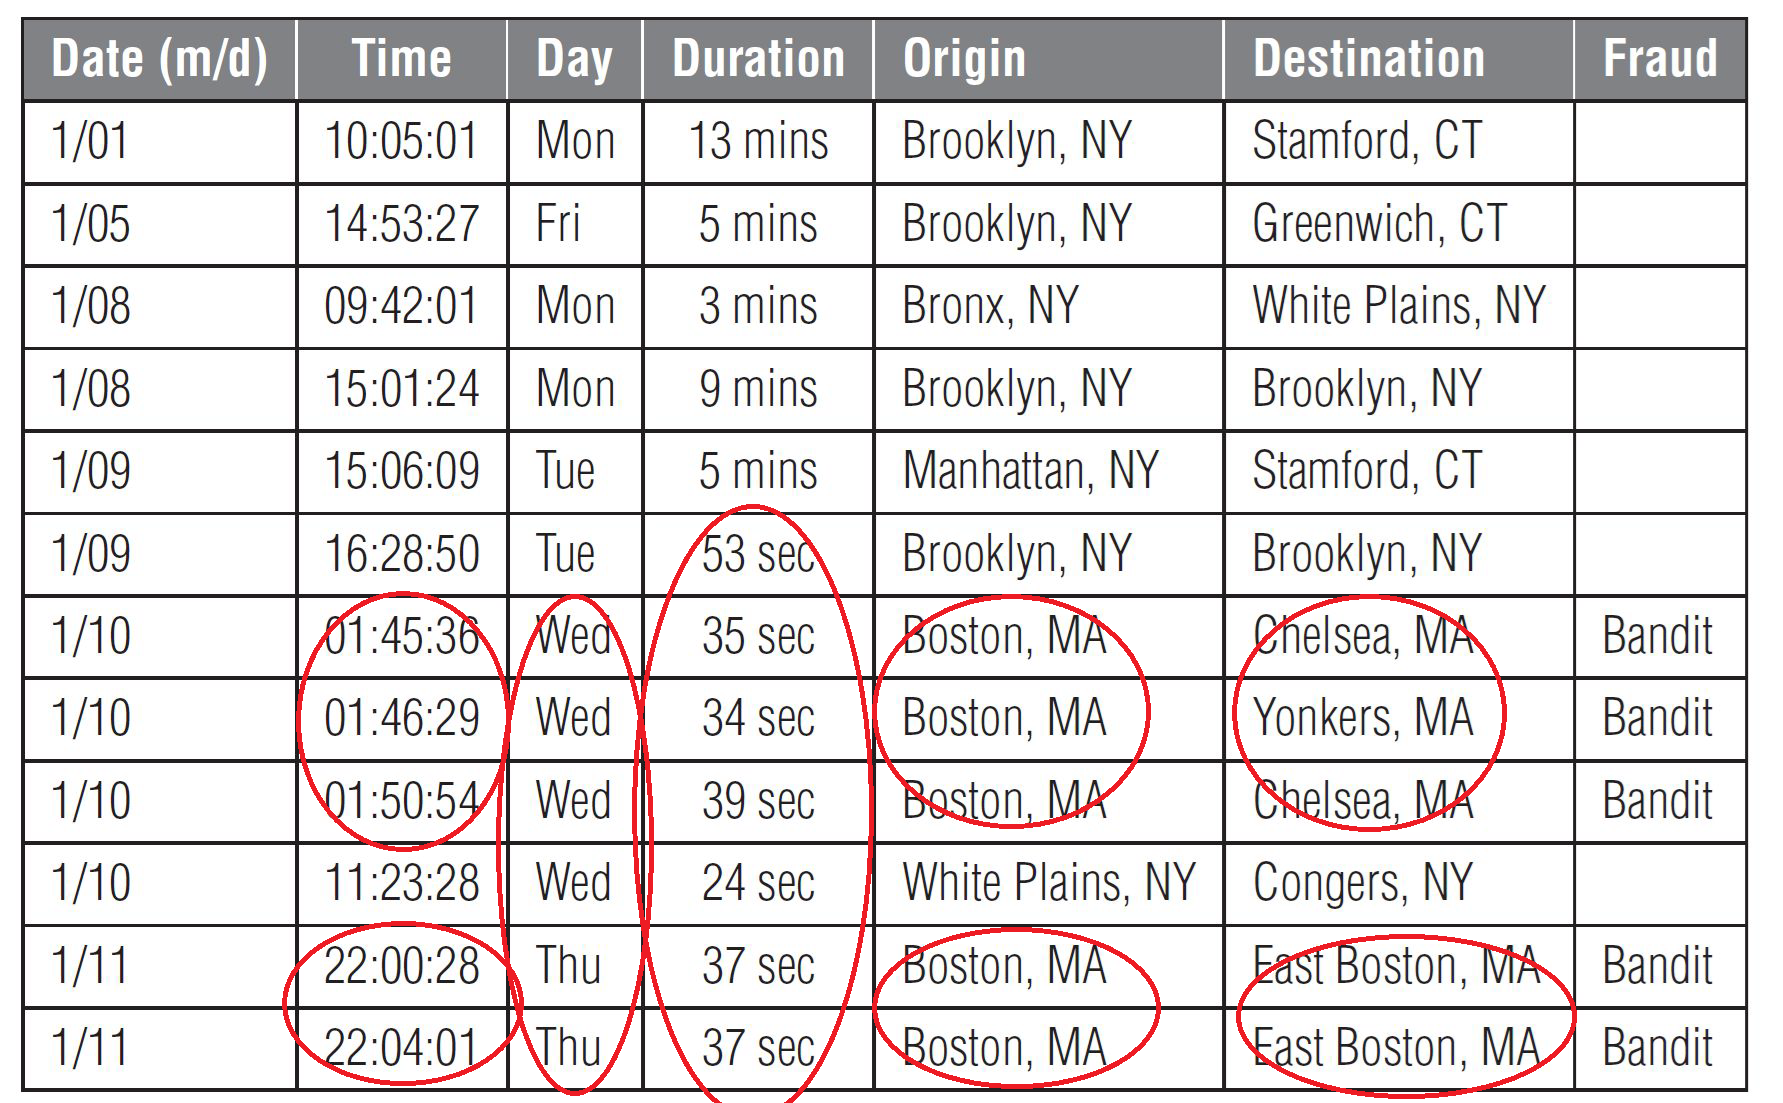
\includegraphics[width=0.6\linewidth]{telecom.png}
            \end{figure}
        \subsubsection{Limitations of unsupervised techniques}
            They are prone to \textbf{deception}\footnote{inganno}: camouflage-like fraud strategies, because it detect new frauds only if them lead to detectable deviations from normality.\\
            These techniques need to be improved by complementing other tools.
    \subsection{Supervised learning techniques}
        Or predictive analytics.\\
        \textit{Learn from historical observations to retrieve patterns that allow differentiating normal and fraudulent behavior}\\
        Aim at finding tracks that fraudsters cannot hide: \textit{"known alarms"}.
        These techniques can be applied to:
        \begin{itemize}
            \item Predict frauds 
            \item Detect frauds 
            \item Estimate the amount of fraud 
        \end{itemize}
        \subsubsection{Limitations of supervised techniques}
            \begin{itemize}
                \item They need historical examples to learn from \textit{(i.e. a labeled dataset)}
                \item They have low detection power against different and new fraud types
            \end{itemize}
    \subsection{Complementarity of supervised and unsupervised methods }
        Use both methods in developing a powerful fraud-detection and prevention system. Each method focuses on different aspects of fraud.
\iffalse
    you'll get a list of transactions ranked by their anomaly scoring 

    unsupervised learning part is used to optimize the detection capacity.
    supervised + user is used to classify transactions 

Graph/Network analysis 
    Possible to combine the before-tokd sup+unsup with this.
    graphs of interactions between different financial institutions 

Frauds are a dynamic phenomenon (slide 116 sua 13:40 slide 80 nostra)
Good detection power (continua)
    reduce as much as possible false positive, because the code means it was written by someone paid for "nothing", and clients may feel annoyed and change bank 
    low false alarm rate

Skewness of the data = only a limited number of cases are frauds 
Ago nerpa gliaio

Operational Efficiency 
    Limited amount of time to reach a decision and let a transaction pass or not 
        impacts design of operations IT systems 
        analytical model?

    Must be able to deal with the massive volumes of data.
\fi